% Preamble
\documentclass[../Relazione_circuiti]{subfiles}

% Packages

\graphicspath{{\subfix{../images/}}}

% Document
\begin{document}

\subsection{Analisi preliminare qualitativa}

  \begin{figure}[H]
    \centering

    \begin{subfigure}[b]{0.3\textwidth}
      \centering
      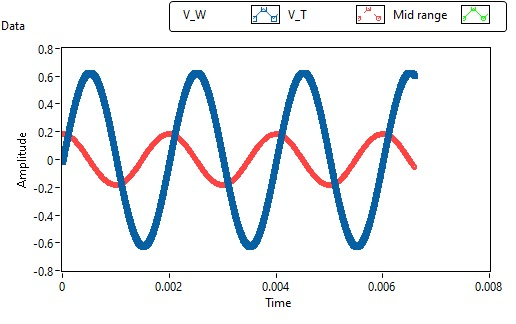
\includegraphics[width=\textwidth]{Cross_waveform_500.jpeg}

      \caption{Segnali a 500Hz}
      \label{fig:signal_500}

    \end{subfigure}
    \begin{subfigure}[b]{0.3\textwidth}
      \centering
      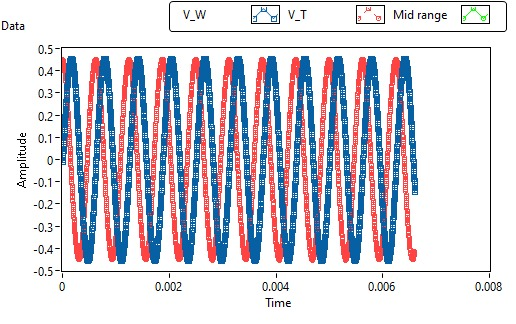
\includegraphics[width=\textwidth]{Cross_waveform_1600.jpeg}

      \caption{Segnali a 1600Hz}
      \label{fig:signal_1600}

    \end{subfigure}
    \begin{subfigure}[b]{0.3\textwidth}
      \centering
      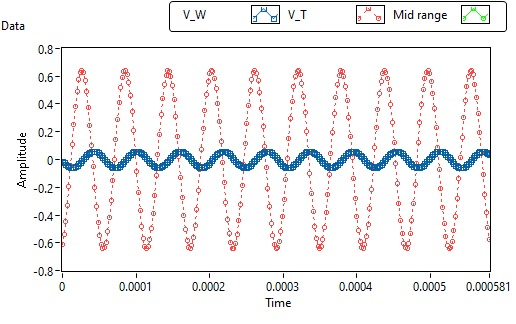
\includegraphics[width=\textwidth]{Cross_waveform_17000.jpeg}

      \caption{Segnali a 17kHz}
      \label{fig:signal_17k}

    \end{subfigure}
    \hfill

    \caption{Segnali osservati sui rami Woofer (blu) e Tweeter (rosso)
      a frequenza fissata.}
    \label{fig:signal_waveforms}

  \end{figure}

  La figura \ref{fig:signal_waveforms}
  mostra la forma d'onda dei segnali osservati sui rami Woofer e Tweeter in risposta ad un segnale sinusoidale. La
  figura \ref{fig:signal_1600} mostra il comportamento nei pressi della frequenza di cross attesa, la figura
  \ref{fig:signal_500} a 1/3 e la figura \ref{fig:signal_17k} a circa 10 volte.

  Si osserva (Figura \ref{fig:signal_1600}
  ) che, coerentemente con quanto atteso, i segnali hanno ampiezza simile nei pressi di $f_{cross}$
  . A basse frequenze si osserva (Figura \ref{fig:signal_500}) un'attenuazione del 60\%
  dell'ampiezza sul ramo Tweeter e nessuna alterazione sul Woofer, ad alte frequenze un'attenuazione sul Woofer
  dell'86\% e nessuna sul Tweeter (Figura \ref{fig:signal_17k}).

\subsection{Analisi della frequenza misurata}

\subsection{Analisi dell'ampiezza}

\begin{figure}[H]
\centering

\begin{subfigure}{=0.7\textwidth}

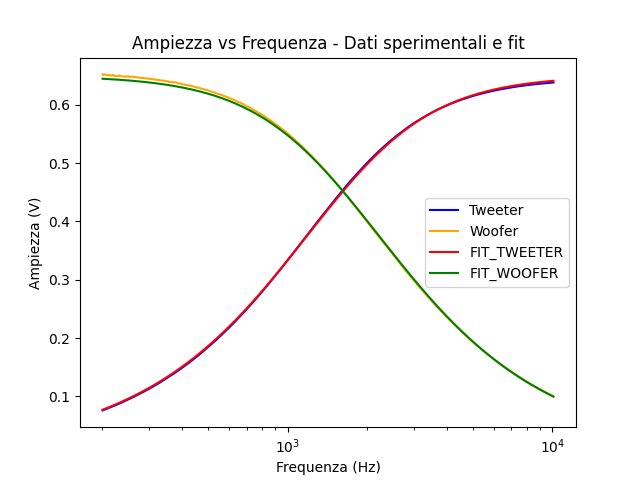
\includegraphics[width=\textwidth]{cross.png}

\end{subfigure}

\caption{Ampiezza misurata in funzione della frequenza (asse della frequenza in scala logaritmica). A causa della scala le incertezze sulle singole misure non sono visibili. L'andamento è rappresentato da una linea continua a causa dell'alta densità di punti.}
\label{fig: cross_amplitude}

\end{figure}

La figura \ref{fig: cross_amplitude} mostra l'andamento di ampiezza dei segnali filtrati in funzione della frequenza. 

La relazione funzionale Ampiezza massima-Frequenza (misurata ai capi della resistenza di carico dei rami) è data da:

\begin{equation}
V_{woofer} = \frac{V_{in}}{\sqrt{R^2+(\omega L)^2}}
\end{equation}

\begin{equation}
V_{tweeter} = \frac{V_{in}}{\sqrt{R^2+(\frac{1}{\omega C})^2}}
\end{equation}

dove $V_{in}$ rappresenta la tensione in ingresso (assunta costante) pari a 0.65, osservata nel ramo Woofer nel limite di basse frequenze e nel ramo Tweeter nel limite di alte frequenze.

E' stato effettuato un fit ai parametri L e C (R assunta costante). Da essi è stata poi ricavata la frequenza di crossover secondo l'Eq. \ref{eq:f_cross}. 

\begin{tabular}{c | c }

%Heading
Grandezza & Valore \\

L & $(10.13 \pm 0.01)$ mH \\
C & $(953.39 \pm 0.05)$ nF

\end{tabular}

\subsection{Analisi della fase}

\end{document}